\documentclass[twocolumn]{article}
\usepackage{graphicx}

\usepackage{cite}
\usepackage{float}
\usepackage[hmarginratio=1:1, margin=1.0in, top=0.5in, bottom=0.5in]{geometry}
% uncomment below to save space
\usepackage[small,compact]{titlesec}

\usepackage[hang, small,labelfont=bf,up,textfont=it,up]{caption} % Custom captions under/above floats in tables or figures
\usepackage{titlesec} % Allows customization of titles
\usepackage{titling} % Customizing the title section
\usepackage{subcaption}
\usepackage{amsmath}
\usepackage{hyperref}
\usepackage{url}
\usepackage{flushend}
\graphicspath{	{figures/}}

\title{\vspace{-0.25in}Fare Share: Flow and Efficiency in NYC's Taxi System}

\author{
\normalsize{\textbf{Abraham Neuwirth}}\\ 
\small Touro College \\ 
\small abraham.neuwirth@student.touro.edu
\and 
\normalsize{\textbf{Fatima Chebchoub}}\\ 
\small NYC College of Technology\\ 
\small fatima.chebchoub@mail.citytech.cuny.edu 
\and 
\normalsize{\textbf{Jai Punjwani}}\\
\small Adelphi University\\
\small jaipunjwani@mail.adelphi.edu 
\and 
\normalsize{\textbf{Marieme Toure}}\\ 
\small NYC College of Technology\\ 
\small marieme.toure@mail.citytech.cuny.edu
}
\date{\vspace{-5ex}}
\begin{document}
\twocolumn[
\begin{@twocolumnfalse}
\maketitle

\end{@twocolumnfalse}
]
\section{Introduction}
New York City is home to millions of people who rely on its robust transportation system. The taxi transportation system in particular plays a critical role in keeping people moving throughout the city. With access to information about every single trip that occurred in a yellow taxi in 2013, we were able to deepen our understanding of how people move throughout the entire city. We were also able to analyze the roles of drivers in the taxi system, and found some interesting ways to improve transportation in New York City. 

\section{Data and Methods}
We used data that was released by the NYC TLC after an initial Freedom of Information Law (FOIL) request by Chris Whong~\cite{Whong:2014}. Although more recent data was available, we used data from 2013 because it contained an anonymized driver’s license for each trip. This information allowed us to associate trips with drivers and analyze their behavior. Due to the overwhelming size of that data, we chose to work with the month of July as a sample month for our analysis.

For each trip, we had relevant information such as the start and end time, pickup and dropoff coordinates, fare paid, distance traveled, total trip time, mode of payment, rate code, and more.

We joined this data with daily weather data obtained from NOAA~\cite{NOAA:2016} to help in our analysis. 
\subsection{Flow}
First, we looked at the overall flow of taxis in NYC to find the general trends that define the movement of people within the city. To understand flow, we mapped geographical coordinates of trips to neighborhoods and then grouped trips by neighborhood. For each neighborhood, we looked at the change in population (number of passengers that entered minus number of passengers that left) at every hour for all weekdays in July. We then used the median change in population of each hour to represent the net flow. Figure~\ref{fig:7am} and figure~\ref{fig:7pm}, which show the net flow for 7 AM and 7 PM respectively, for weekdays in July, help us visualize the movement of people and understand the flow in NYC.

While this snapshot is certainly informative in its own right, it betrays the level of detail and intricacy of the data at hand. Different people live in different neighborhoods, and each of these neighborhoods have their own story to tell. To tease out these stories, we grouped all the rides by source neighborhood, time of the week (weekends and weekdays) and hour of day, and for each group we computed the distribution of probability for each possible destination. We then built a tool~\cite{DS3:2016} which allows one to explore this data to see trends of popular destinations for individual neighborhoods at different times. 


\begin{figure}[h]
 
\begin{subfigure}{0.5\textwidth}
\centering
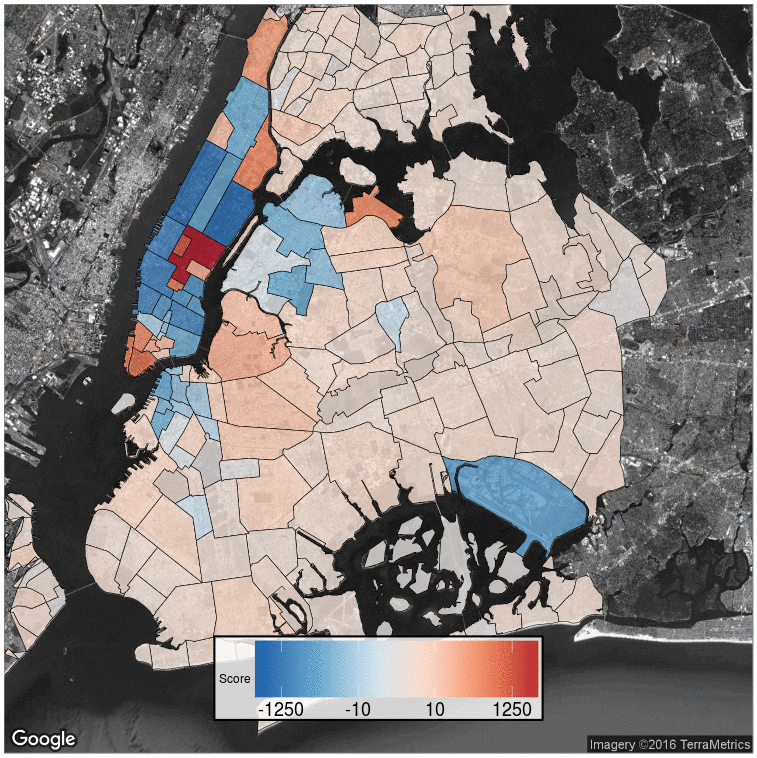
\includegraphics[width=0.75\linewidth]{7am} 
\caption{7 AM}
\label{fig:7am}
\end{subfigure}
\begin{subfigure}{0.5\textwidth}
\centering
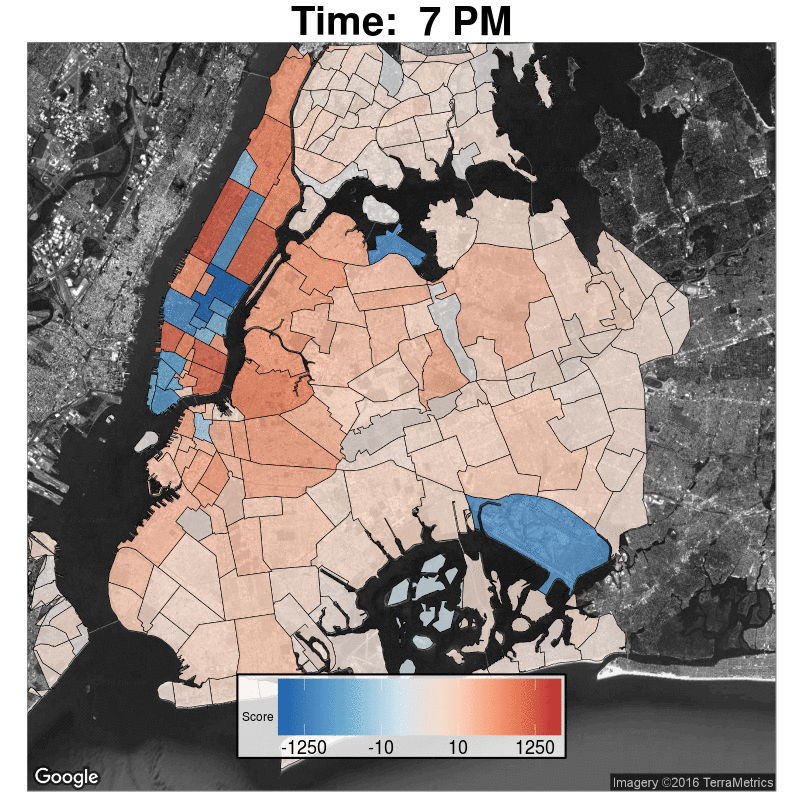
\includegraphics[width=0.75\linewidth]{7pm}
\caption{7 PM}
\label{fig:7pm}
\end{subfigure}
 
\caption{Net Flow of people during weekdays in July '13}
\label{fig:flow}
\end{figure}

\section{Driver and Shift Efficiency}
Next, we tried to understand the role of drivers in the taxi system. In particular, we wanted to answer two questions:

(1) How do driver earnings vary?
(2) Is that variation due to chance?

By answering these questions, we can assess whether or not drivers have significantly varying skill levels. We began by trying to determine the efficiency of a driver in a work period. We defined efficiency as the ratio of the total metered fare earned in a work period to the total work time. The total metered fare was information we obtained directly from our data by summing up the metered fare for each driver for his trips. However, the data did not contain the time each driver spent working in a shift; rather, it only had records of when each driver drove with a passenger. Previous work used the distance between a dropoff and the next pickup~\cite{LEE:2015} to approximate total shift time. We tried to take a more systematic approach to determine a driver's shift by looking at the downtime (time between a drop off and the next pickup) for all trips. Figure~\ref{fig:downtime_distribution} shows the distribution of downtimes for all drivers. 

\begin{figure}[h]
  \centering
  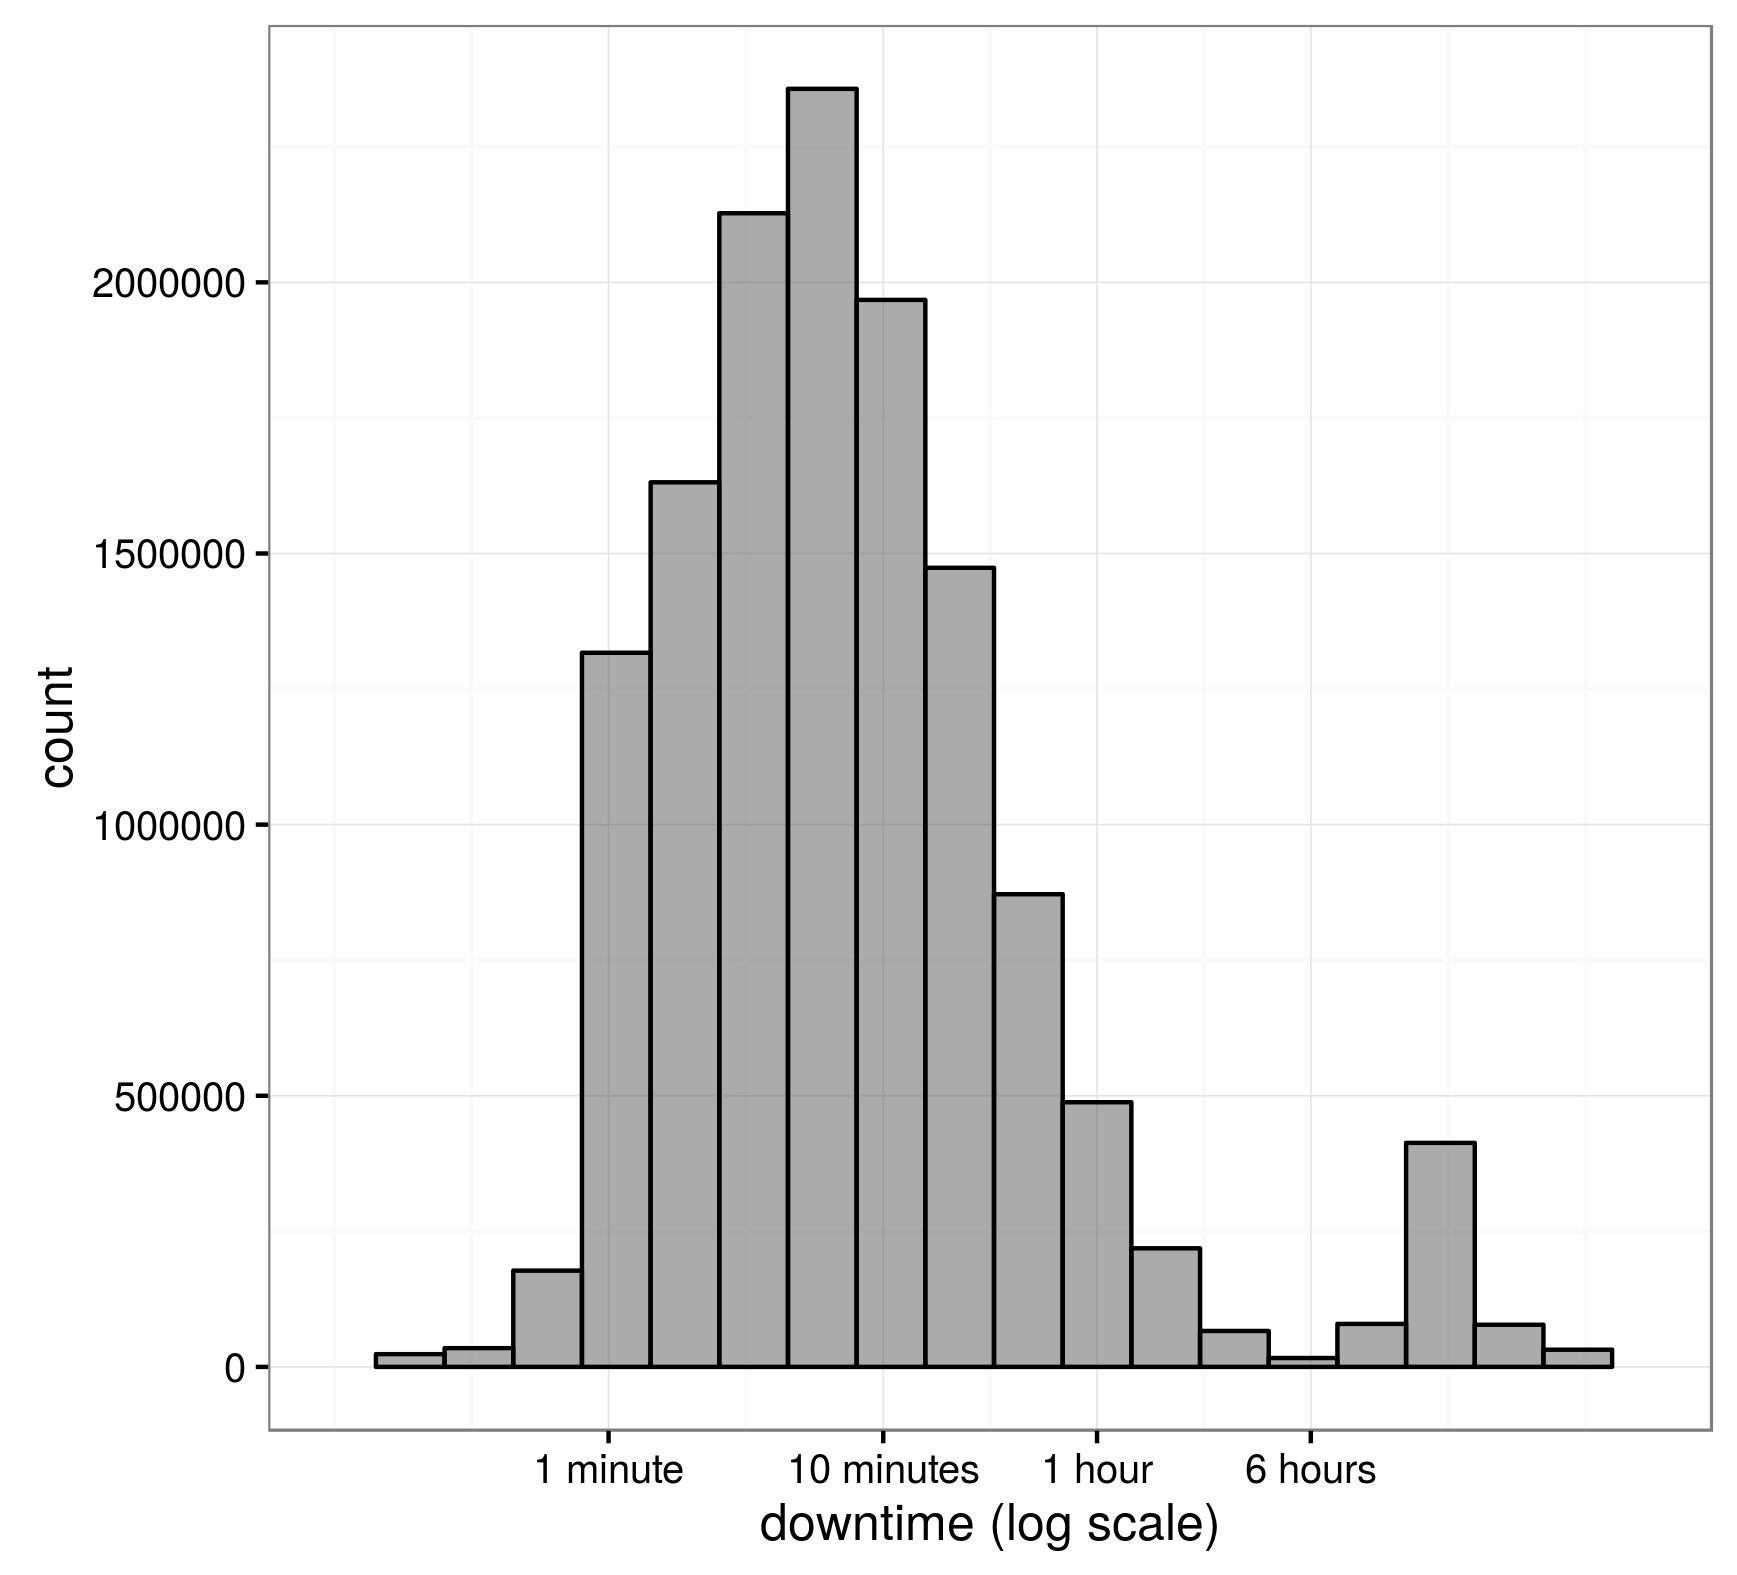
\includegraphics[width=.9\linewidth]{downtime_distribution}
  \captionof{figure}{Downtimes for all rides. We see that there are very few drivers who have a 6-hour gap between two rides.}
  \label{fig:downtime_distribution}
\end{figure}

Looking at this distribution, we defined the end of a shift at the last drop off when there is no driver activity for at least six hours. This corroborates previous research on shift time~\cite{Farber:2014}. The next pickup marked the beginning of the next shift. With this shift information, we were able to group each driver's rides into shifts and compute the efficiency for each shift.

Now, we wanted to find out what effect the driver has on the efficiency of shifts. To accomplish that, we ran a linear regression, using the following model: 

\begin{eqnarray*}
&& \beta_{\mathrm{driver~id}} + \beta_{\mathrm{hour}} + \beta_{\mathrm{weekend}} + \beta_{\mathrm{hour:weekend}} + \\
  & & \gamma_p x_p + \sum_{n=1}^N \rho_n p_n + \sum_{n=1}^N \delta_n d_n
\end{eqnarray*}

Here, each $\beta$ represents the effect of its corresponding subscript, whether it be the driver’s ID, the start hour of a shift, or whether it is a weekend of the weekday. $x_p$ is precipitation in inches, and  $\gamma_p$ is its coefficient. The two summations represent the percentage of pickups ($p_n$) and drop-offs ($d_n$), respectively, in each neighborhood, with $\rho$ and $\delta$ as their cooefficients.

We also ran the same model on a dataset with shuffled driver IDs; that is, each driver was randomly assigned shifts, which had varying efficiencies. In the randomized model, drivers' efficiencies were normally distributed, with the most extreme outliers making within $\pm$$\$$5/hour from the center. In the nonrandomized model, drivers' efficiencies varied more, with the most extreme outliers consistently making $\pm$$\$$10/hour. This information is summarized in figure~\ref{fig:efficiency}.
\begin{figure}[h]
  \centering
  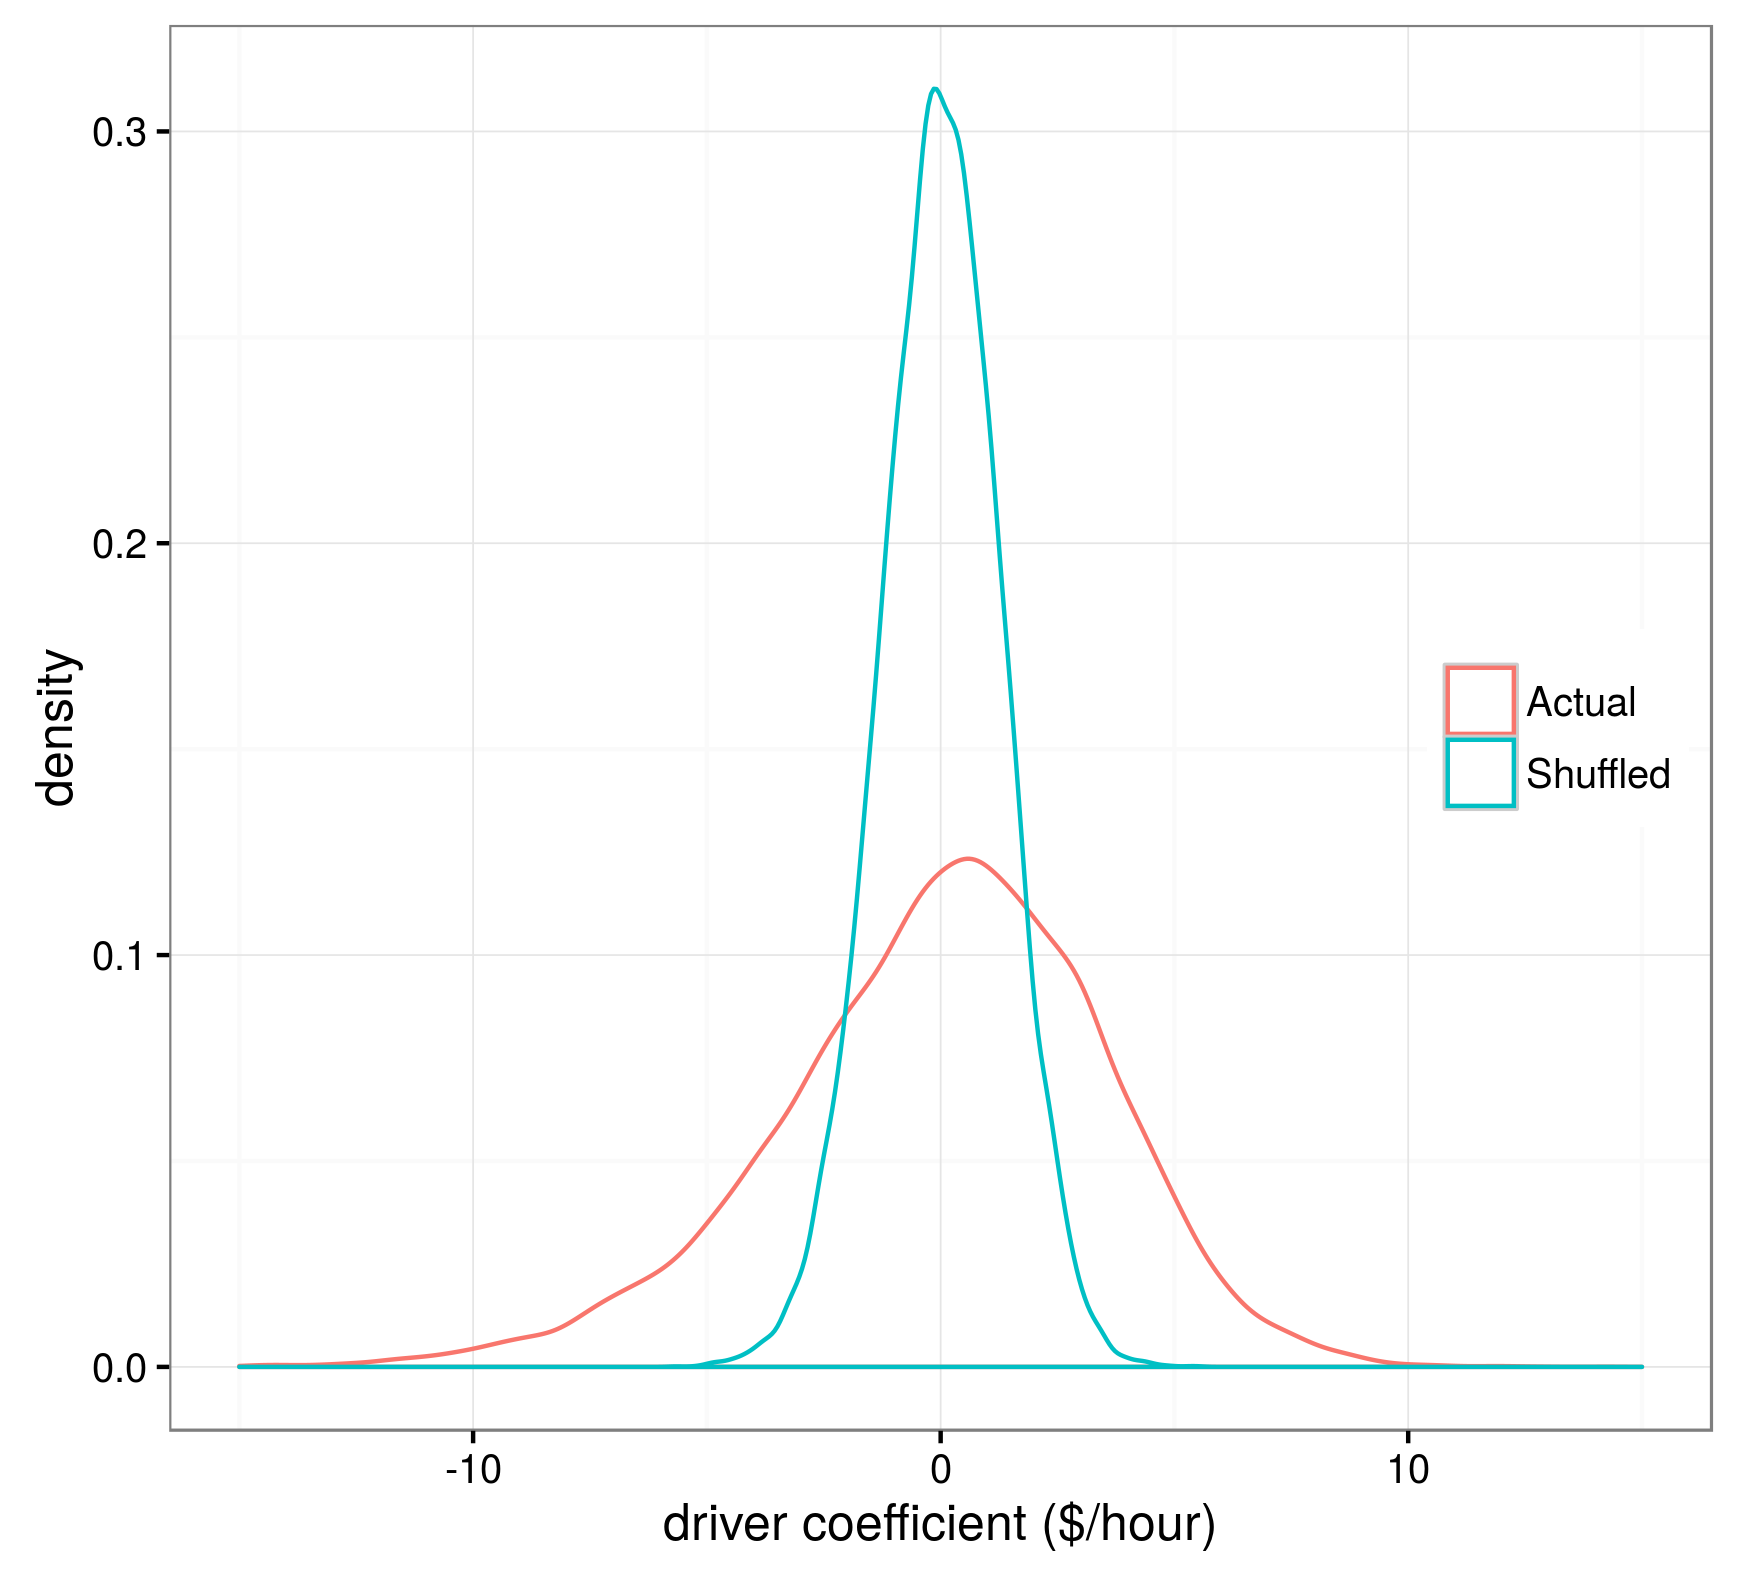
\includegraphics[width=.9\linewidth]{efficiency}
  \captionof{figure}{Effect of Driver ID on Efficiency}
  \label{fig:efficiency}
\end{figure}
This distribution reveals that there is a significant variation in drivers’ earnings, and that this variation is not due to chance. Thus, there is a strong correlation between the driver and the efficiency of a given shift. Anyone can be a taxi driver, but there are certain skills that distinguishes one drivers from others! 
\section{Carpooling}
After looking at flow and driver behavior, we wanted to find ways to improve the overall taxi system. Past work have focused on recommender systems~\cite{ZHAN:2014} or information systems~\cite{KIM:2005}, which would require taxi drivers to be notified via a mobile application or a similar solution. We take a different approach and look at a policy that can be implemented at existing taxi stands, with little overhead. We noticed that there were lots of trips occurring between similar locations. As a result, we considered a scenario in which people would carpool. Our thought experiment made the following assumptions: Customers would be willing to (1) share a cab with strangers, (2) wait up to five minutes to find someone to carpool with, (3) walk up to one block, (4) share a destination within ~1 kilometer of their own destination. We also assumed that customers would carpool only for trips between two distinct neighborhoods, because customers would probably not want to wait for trips that are relatively short.

To look for carpooling potential, we looked for trips that started in a neighborhood X within 1 block from each other, and ended in a neighborhood Y within a 1 km radius. We looked at such trips in 5-minute bins. As we were hoping, a significant number of trips were taking place around the same location, at a similar time. After finding these trips and plotting their pick-up points on a map, we identified the top carpooling hotspots in NYC (figure~\ref{fig:hotspots}). Unsurprisingly, many of these places are either major transportation hubs (JFK airport, LaGuardia airport, Penn Station, Port Authority Bus Terminal, and Grand Central Terminal) or popular cultural attractions (the Metropolitan Museum of Art, the Lincoln Center, the Theater District, etc.). 
\begin{figure}[h]
  \centering
  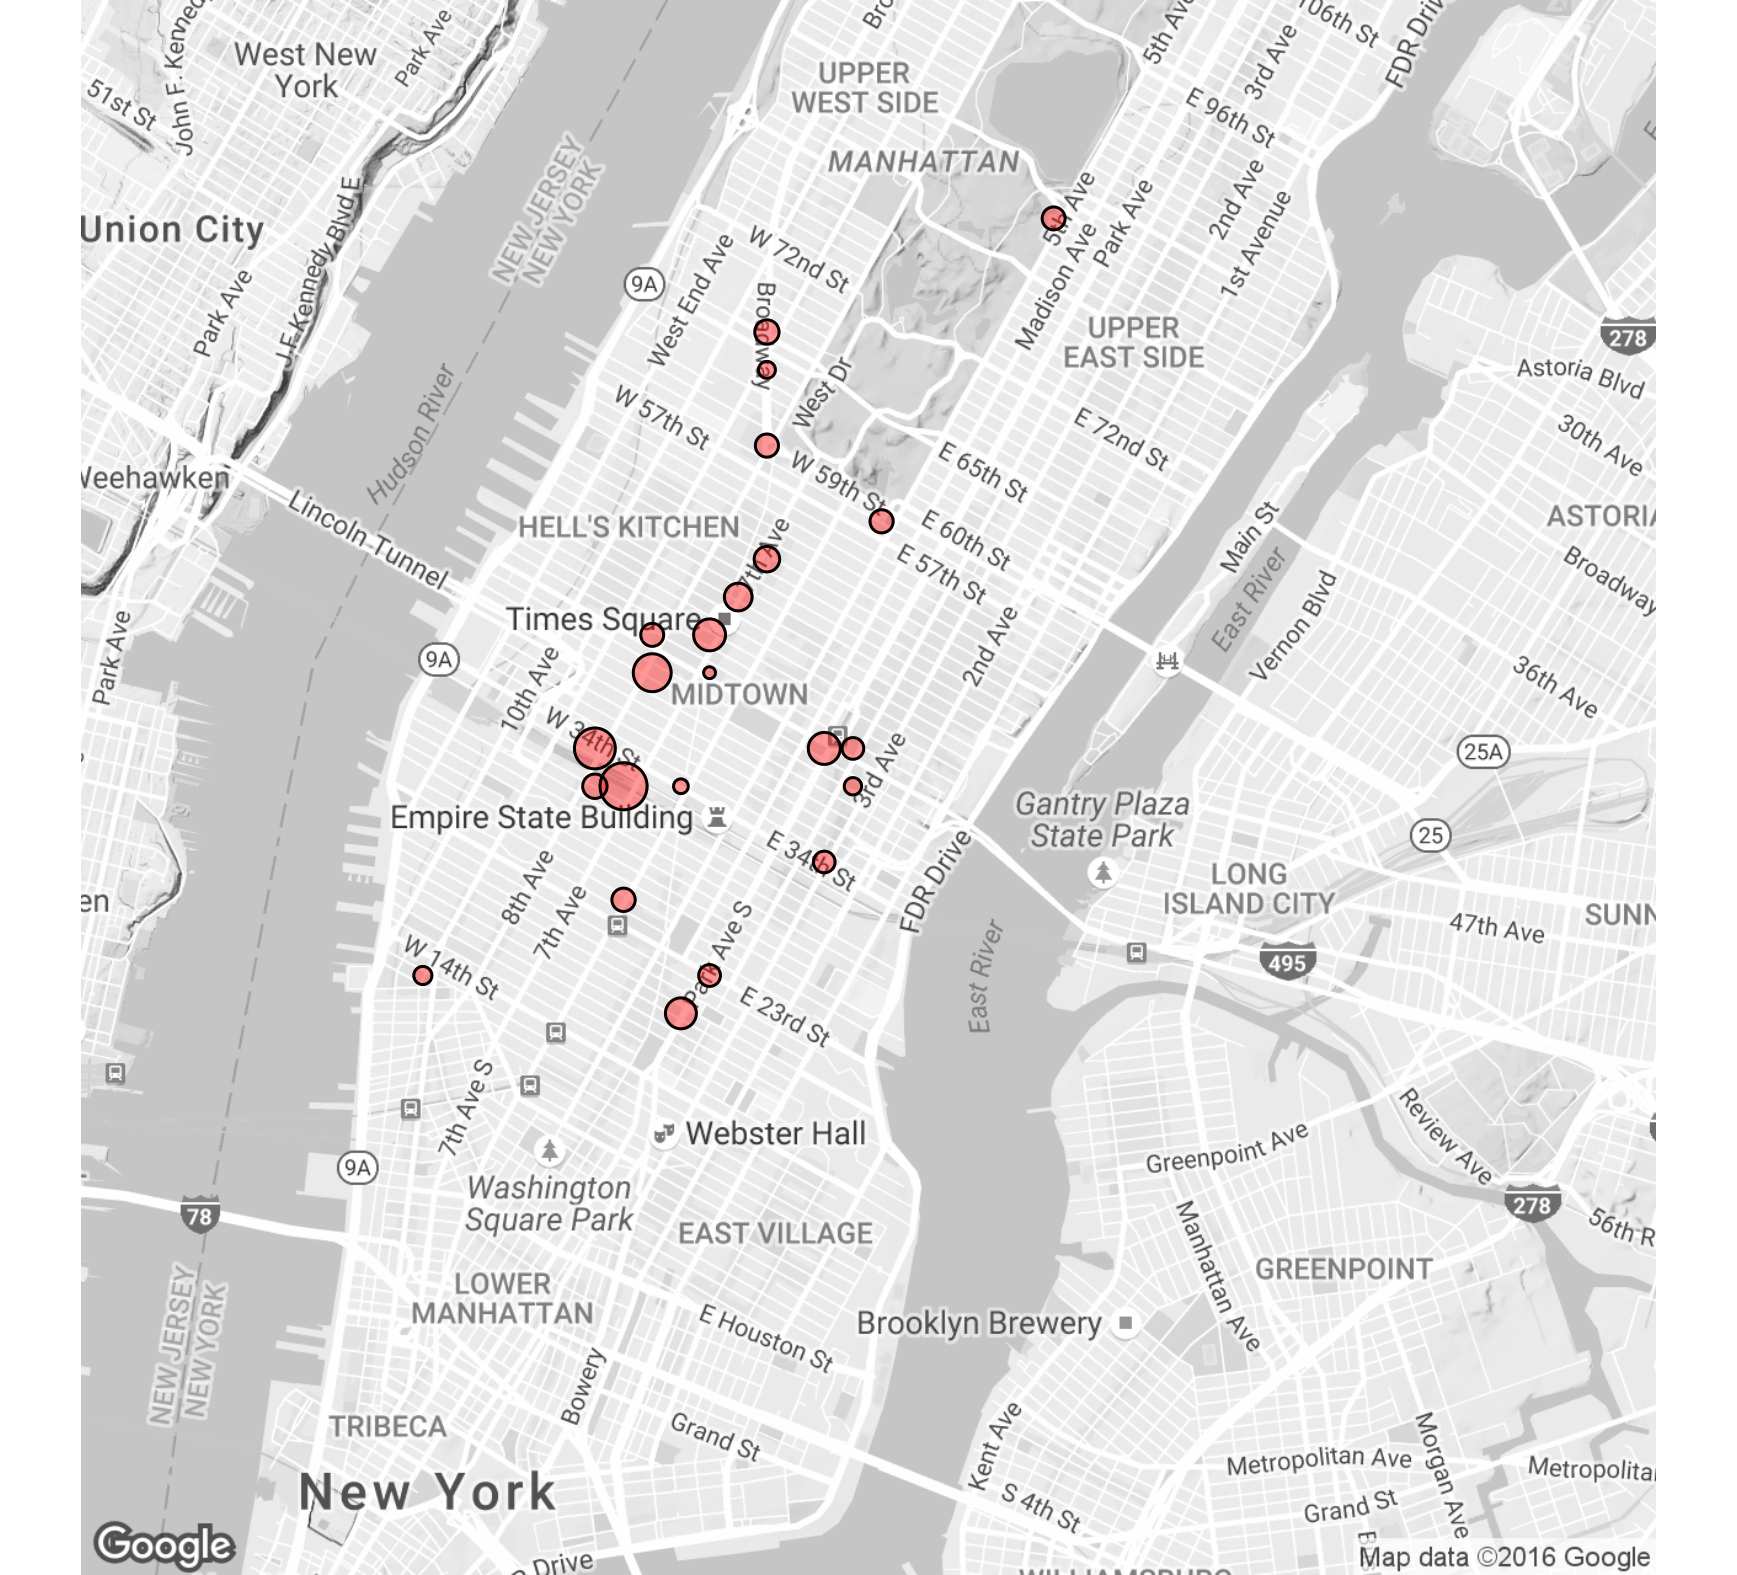
\includegraphics[width=.9\linewidth]{top_25_hotspots}
  \captionof{figure}{Top carpooling hotspots in Manhattan. Points are sized by how frequent a carpooling potential occurs at a location.}
  \label{fig:hotspots}
\end{figure}

Next, we calculated our potential savings. For each hotspot, we calculated the minimum number of cabs by assuming that up to 4 passengers (92\% of taxis fit 4 passengers~\cite{TLC:2007}) would fit in one cab. Since each cab essentially makes one trip, we equated the minimum cabs needed to the minimum number of trips that would be made. Thus, we subtracted the minimum number of trips from the actual number of trips that were made to see how many trips we could cut down. We then computed the possible fare that could be saved by multiplying the number of trips saved by the average fare of all trips. Our potential savings over the month of July were around 5\% of the trips and 6\% of total money spent by customers.

We also found that with less restrictive assumptions, i.e. widening the waiting period to 6 minutes, and including rides taking place within the same neighborhood, we can improve the savings up to 14\% for the number of rides and fare paid. In addition to saving money, carpooling would also help the environment and reduce traffic! 

\section{Acknowledgements}
We thank our mentors Ashton Anderson (Microsoft Research), Christopher Riederer (Columbia University), Jake Hofman (Microsoft Research), and Siddhartha Sen (Microsoft Research) for their mentorship as a part of the 2016 Microsoft Research Data Science Summer School. Maps were produced using the ggmap package in R~\cite{KAHLE:2013}.

% Bibliography
%\vspace{-0.5em}
\bibliographystyle{unsrt}
\bibliography{refs}
\end{document}
%%% Local Variables:
%%% mode: latex
%%% TeX-master: t
%%% End:
\grid
